\documentclass{article}
\usepackage[a4paper, total={7in, 9.5in}]{geometry}
\usepackage{amsmath,amsfonts,amsthm,amssymb,graphicx,float, setspace, bm}
\usepackage[utf8]{inputenc}
\usepackage{float}
\usepackage{titlesec}
\usepackage{setspace}
\usepackage{geometry}
\usepackage[style=numeric]{biblatex}
\usepackage[autostyle=true]{csquotes}
\usepackage{breqn}
\usepackage{subfig}
\usepackage[bottom]{footmisc}
\usepackage{adjustbox}
\usepackage{lipsum}
\usepackage{hyperref}
\usepackage[ruled,vlined]{algorithm2e}
\hypersetup{
    colorlinks=true,
    urlcolor=magenta
}
\usepackage[table,x11names]{xcolor}

\usepackage{xltabular}
\usepackage{multirow}
\usepackage{booktabs}


\renewcommand{\baselinestretch}{1.5} 
\setlength\parindent{0pt}
%----------------------------------------------------------------------------------------
%	START
%----------------------------------------------------------------------------------------

\newcommand{\horrule}[1]{\rule{\linewidth}{#1}}

\title{ \normalfont \normalsize 
\huge CPSC 532W - Homework 3}
\date{}
\author{Xiaoxuan Liang - 48131163}
\def\cond{\; | \;}

\begin{document}

\maketitle

Public GitHub repo: https://github.com/Xiaoxuan1121/CPSC532W/tree/main/a3
\begin{enumerate}
\item Program 1: the program has been run for 50000 iterations for each method,  and the results are:
\begin{enumerate}
\item Importance Sampling:

\begin{figure}[!ht]
	\centering
	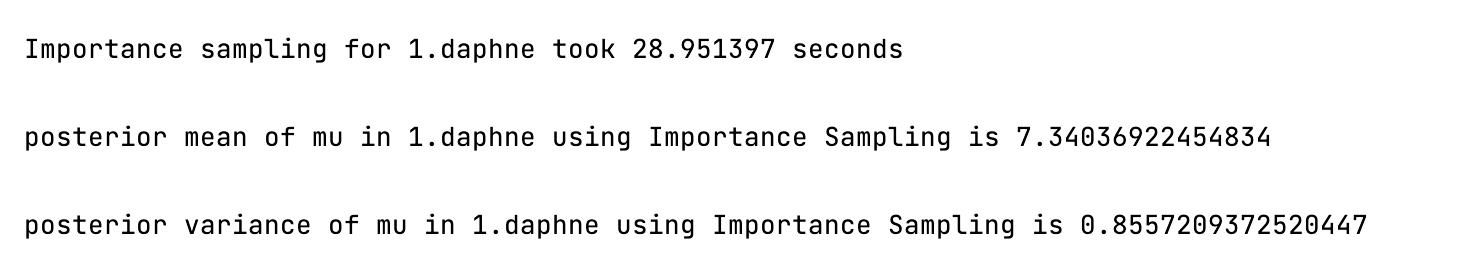
\includegraphics[scale=0.6]{../figs/IS/1_program_results}
\end{figure}

\begin{figure}[!ht]
	\centering
	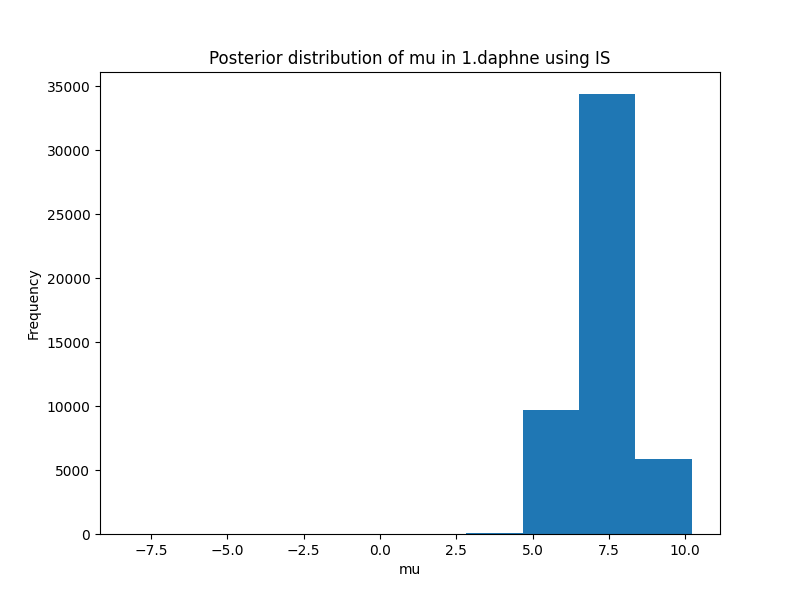
\includegraphics[scale=0.6]{../figs/IS/posterior_histogram_1_daphne}
	\caption{Posterior distrbution for mu for 1.daphne using Importance Sampling}
\end{figure}

\newpage
\item MH Gibbs:

\begin{figure}[!ht]
	\centering
	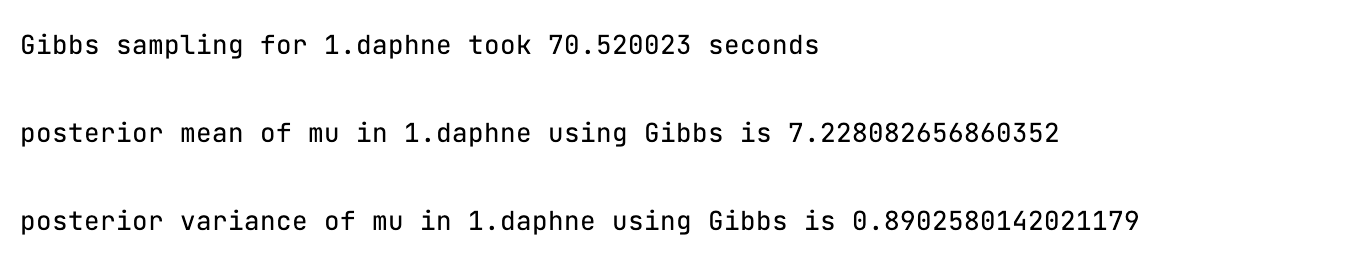
\includegraphics[scale=0.5]{../figs/Gibbs/1_program_results}
\end{figure}

\begin{figure}[!ht]
	\centering
	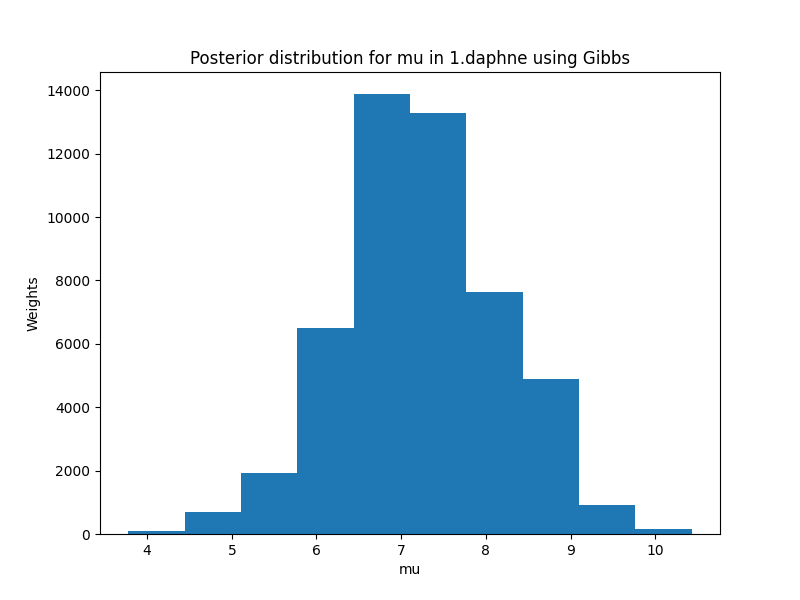
\includegraphics[scale=0.5]{../figs/Gibbs/posterior_histogram_1_daphne}
	\caption{Posterior distrbution for mu for 1.daphne using MH Gibbs Sampling}
\end{figure}


\begin{figure}[!ht]
	\centering
	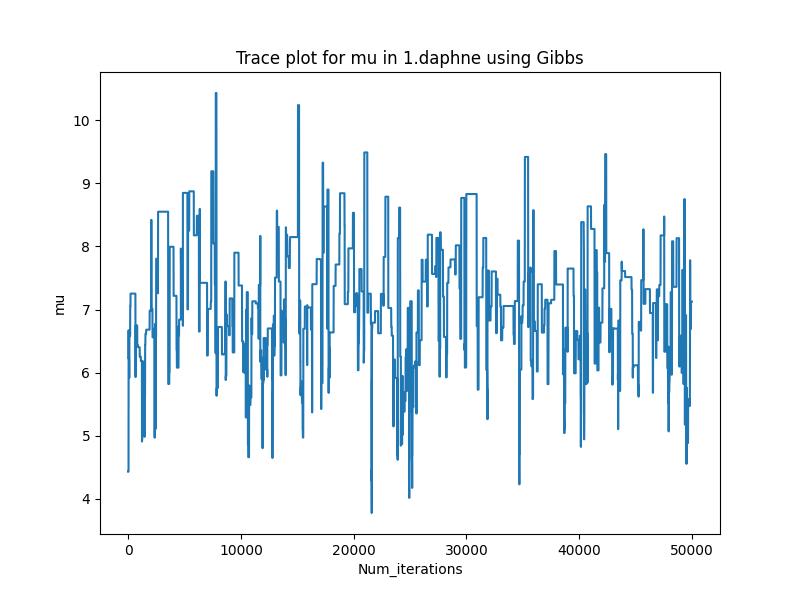
\includegraphics[scale=0.5]{../figs/Gibbs/trace_plot_1_daphne}
	\caption{Trace plot for mu for 1.daphne using MH Gibbs Sampling}
\end{figure}


\begin{figure}[!ht]
	\centering
	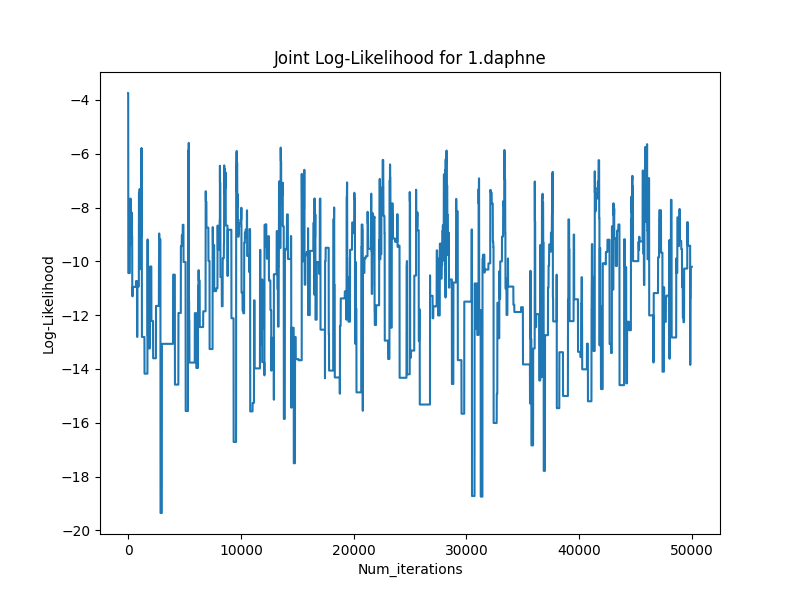
\includegraphics[scale=0.5]{../figs/Gibbs/joint_log_likelihood_1_daphne}
	\caption{Joint loglikelihood plot for mu for 1.daphne using MH Gibbs Sampling}
\end{figure}

\newpage
\item HMC:

\begin{figure}[!ht]
	\centering
	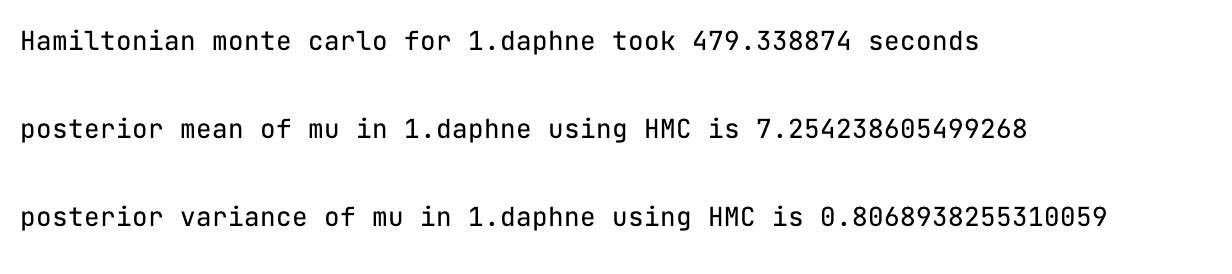
\includegraphics[scale=0.6]{../figs/HMC/1_program_results}
\end{figure}

\begin{figure}[!ht]
	\centering
	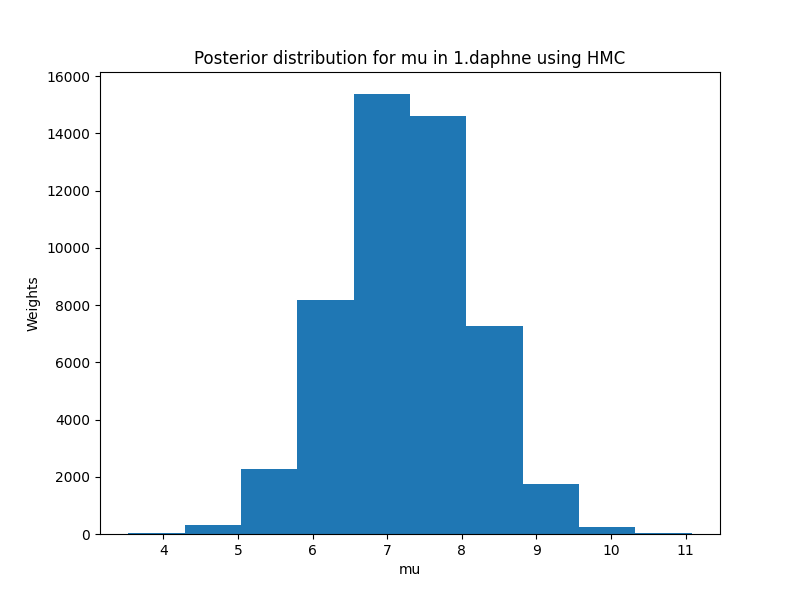
\includegraphics[scale=0.6]{../figs/HMC/posterior_histogram_1_daphne}
	\caption{Posterior distrbution for mu for 1.daphne using HMC}
\end{figure}

\begin{figure}[!ht]
	\centering
	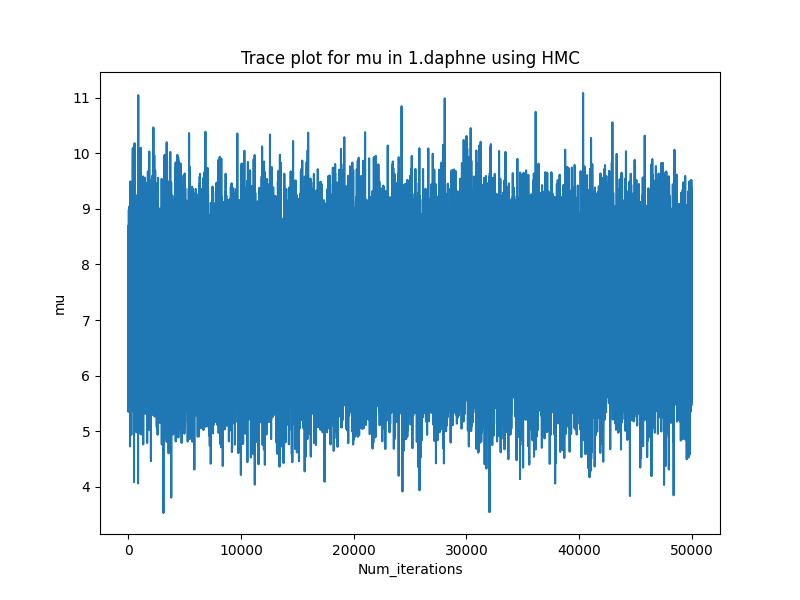
\includegraphics[scale=0.6]{../figs/HMC/trace_plot_1_daphne}
	\caption{Trace plot for mu for 1.daphne using HMC}
\end{figure}


\begin{figure}[!ht]
	\centering
	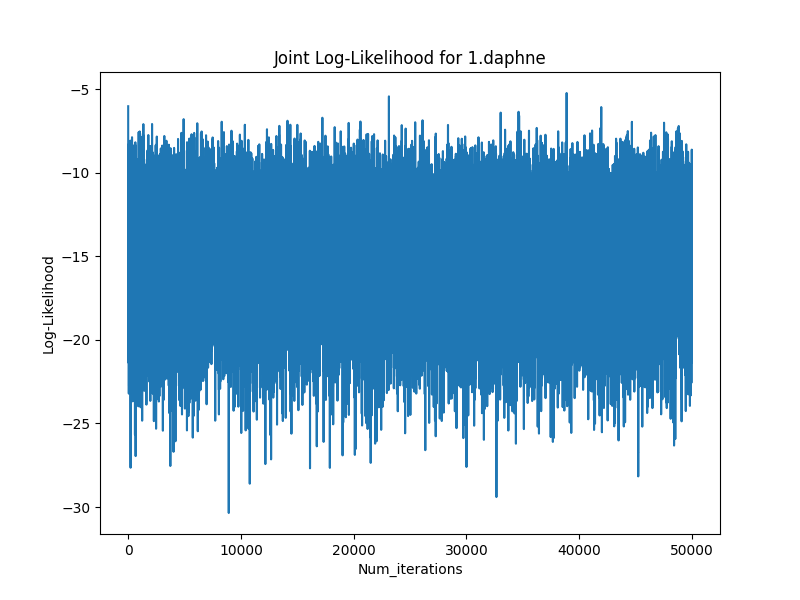
\includegraphics[scale=0.6]{../figs/HMC/joint_log_likelihood_1_daphne}
	\caption{joint loglikelihood plot for mu for 1.daphne using HMC}
\end{figure}
\end{enumerate}


\item Program 2: First two methods were ran 50000 iterations,  HMC is ran 15000 iterations
\begin{enumerate}
\newpage
\item Importance Sampling

\begin{figure}[!ht]
	\centering
	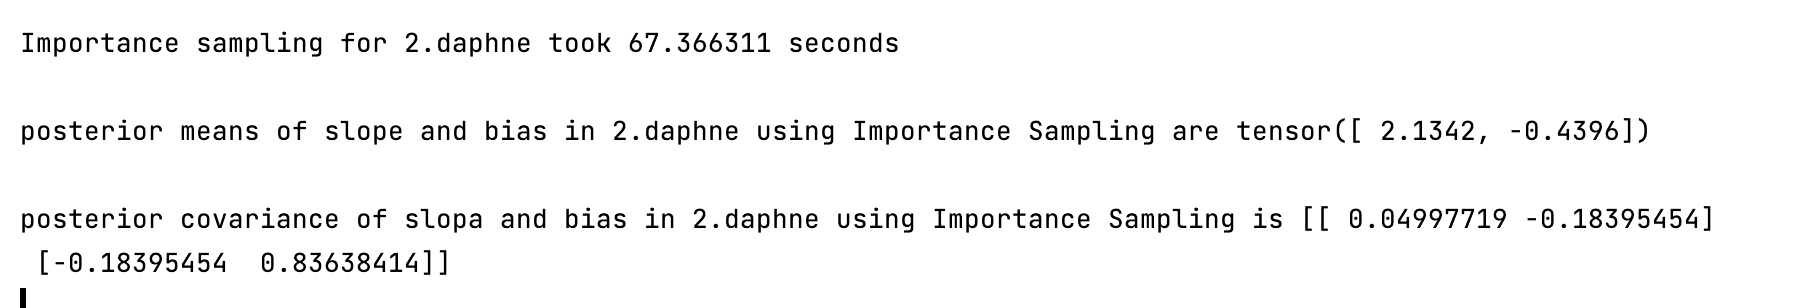
\includegraphics[scale=0.5]{../figs/IS/2_program_results}
\end{figure}

\begin{figure}[!htp] 
    \centering
    \subfloat[Samples from the posterior for slope]{%
        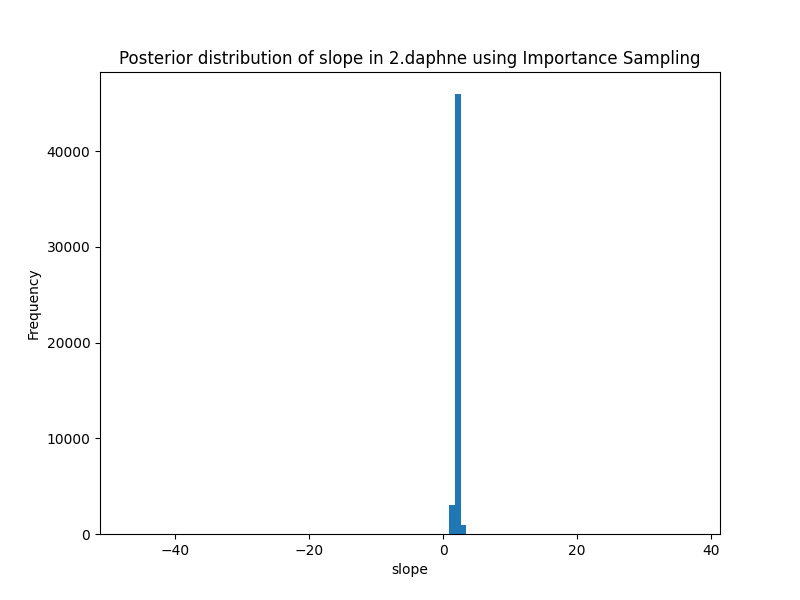
\includegraphics[width=0.5\textwidth]{../figs/IS/posterior_histogram_2_slope__daphne}%
        \label{fig:a}%
        }%
    \hfill%
    \subfloat[Samples from the posterior for bias]{%
        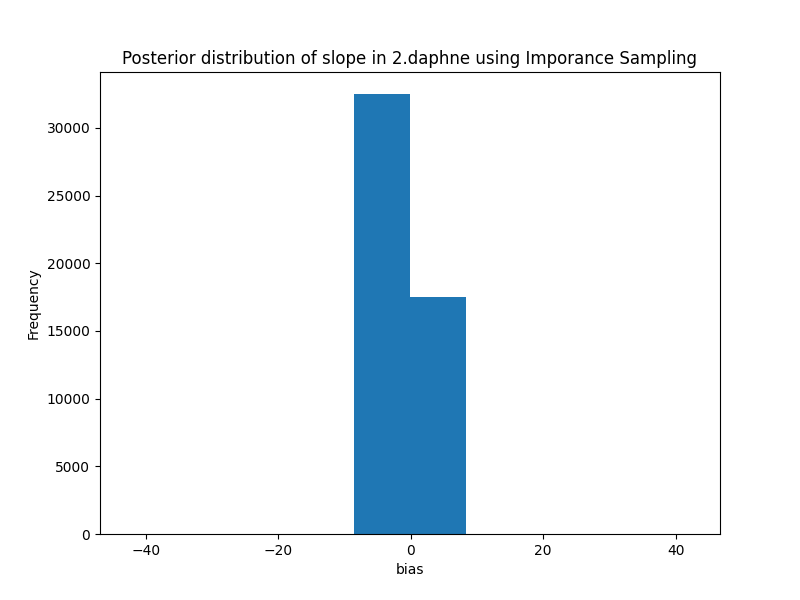
\includegraphics[width=0.5\textwidth]{../figs/IS/posterior_histogram_2_bias__daphne}%%
        \label{fig:b}%
        }%
        \caption{Posterior distribution for slope and bias for 2.daphne using Importance Sampling}
\end{figure}

\newpage
\item MH Gibbs

\begin{figure}[!ht]
	\centering
	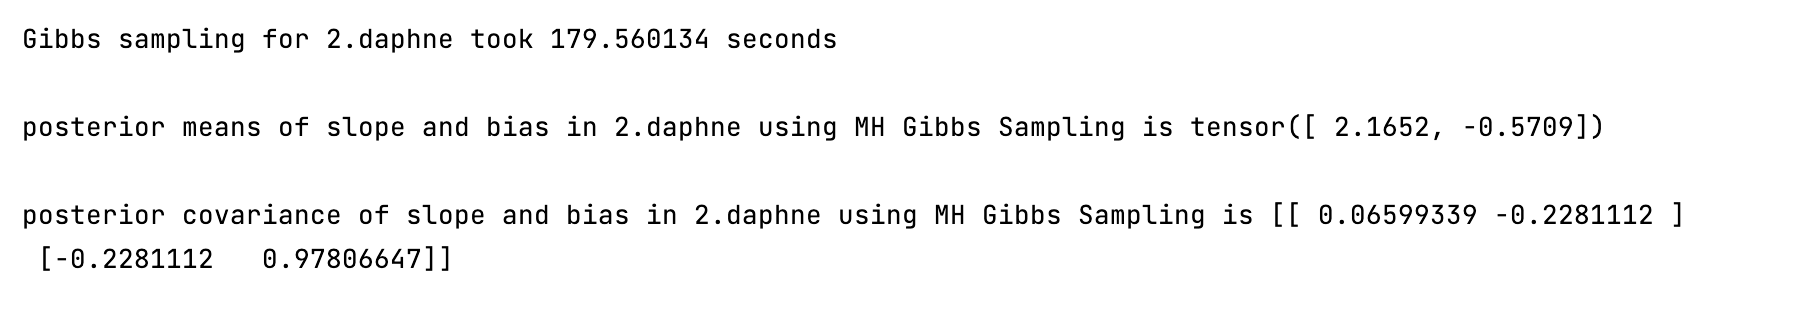
\includegraphics[scale=0.5]{../figs/Gibbs/2_program_results}
\end{figure}

\begin{figure}[!htp] 
    \centering
    \subfloat[Samples from the posterior for slope]{%
        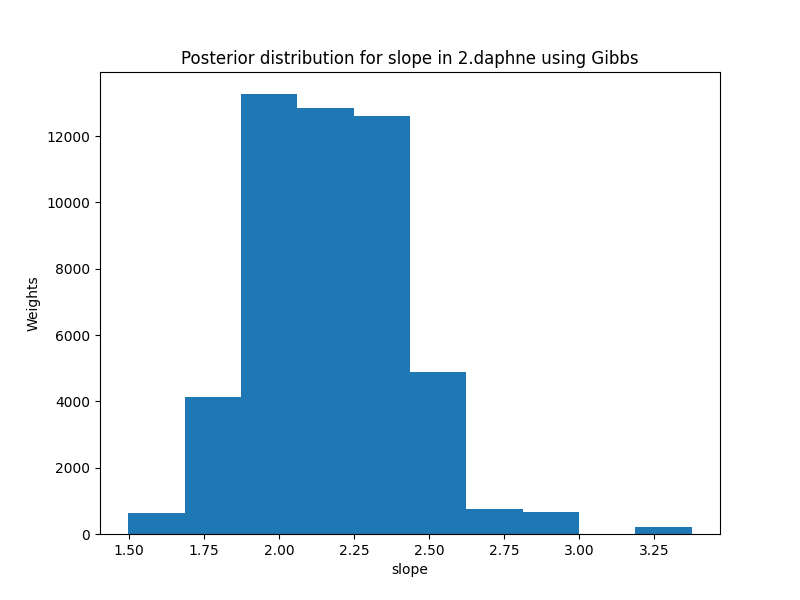
\includegraphics[width=0.5\textwidth]{../figs/Gibbs/posterior_histogram_2_slope_daphne}%
        \label{fig:a}%
        }%
    \hfill%
    \subfloat[Samples from the posterior for bias]{%
        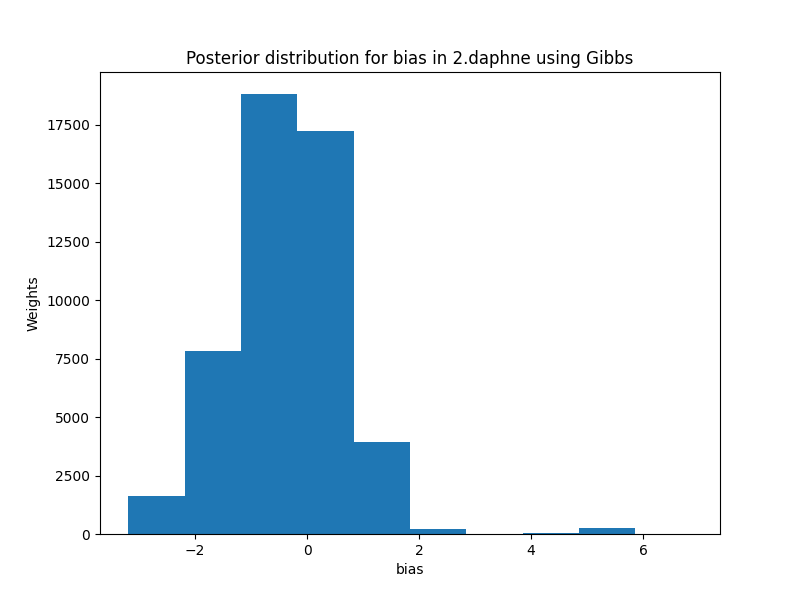
\includegraphics[width=0.5\textwidth]{../figs/Gibbs/posterior_histogram_2_bias_daphne}%%
        \label{fig:b}%
        }%
        \caption{Posterior distribution for slope and bias for 2.daphne using MH Gibbs Sampling}
\end{figure}

\begin{figure}[!htp] 
    \centering
    \subfloat[Samples from the posterior for slope]{%
        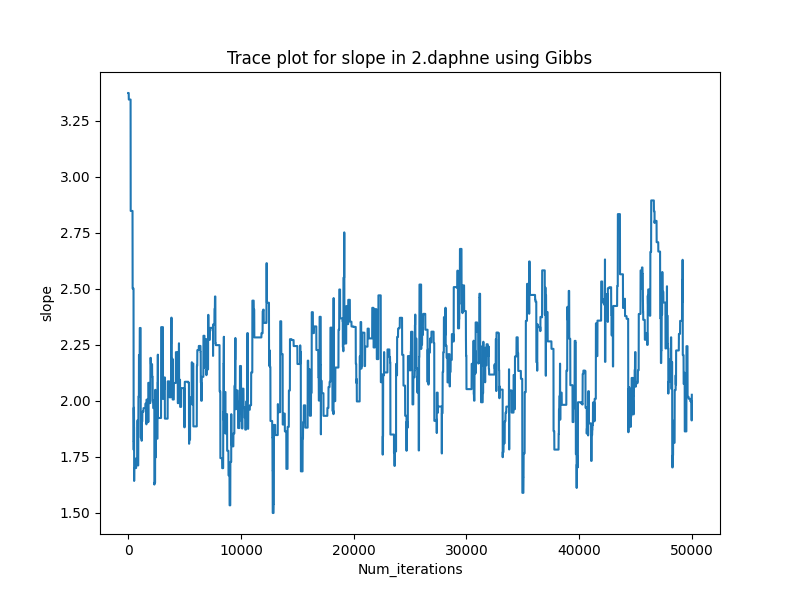
\includegraphics[width=0.5\textwidth]{../figs/Gibbs/trace_plot_2_slope_daphne}%
        \label{fig:a}%
        }%
    \hfill%
    \subfloat[Samples from the posterior for bias]{%
        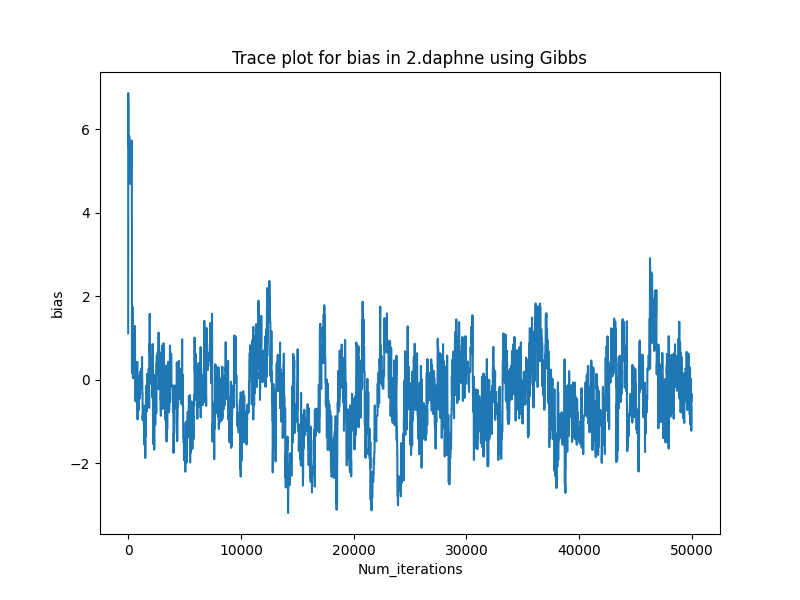
\includegraphics[width=0.5\textwidth]{../figs/Gibbs/trace_plot_2_bias_daphne}%%
        \label{fig:b}%
        }%
        \caption{Trace plots for slope and bias for 2.daphne using MH Gibbs Sampling}
\end{figure}


\begin{figure}[!htp] 
    \centering
    \subfloat[Samples from the posterior for slope]{%
        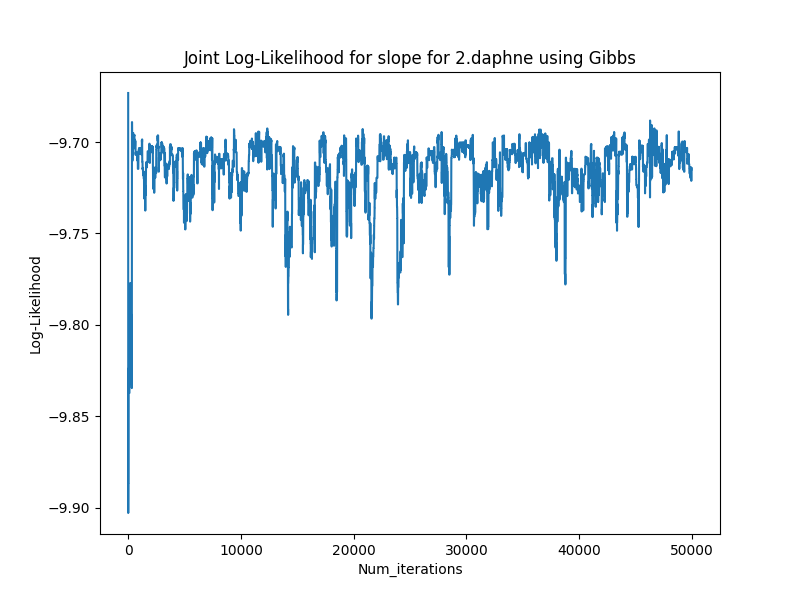
\includegraphics[width=0.5\textwidth]{../figs/Gibbs/joint_log_likelihood_2_slope_daphne}%
        \label{fig:a}%
        }%
    \hfill%
    \subfloat[Samples from the posterior for bias]{%
        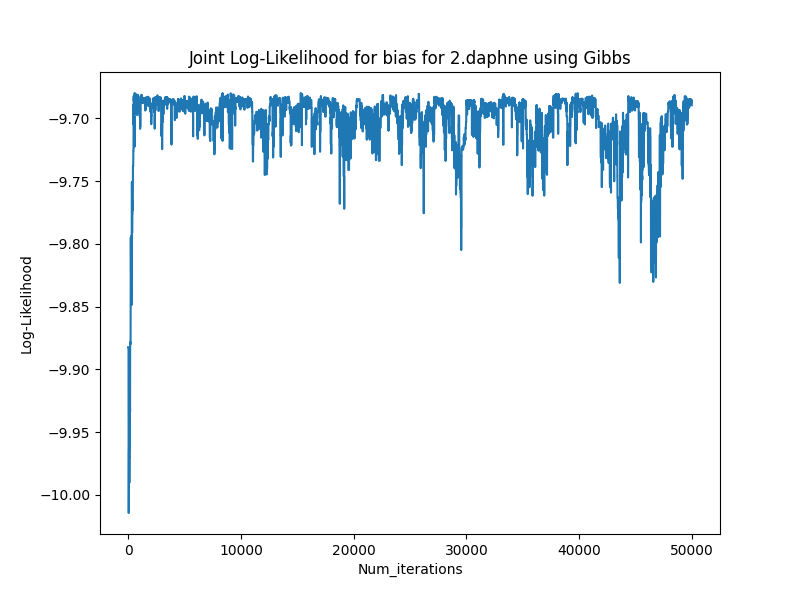
\includegraphics[width=0.5\textwidth]{../figs/Gibbs/joint_log_likelihood_2_bias_daphne}%%
        \label{fig:b}%
        }%
        \caption{Joint Log-likelihood plots for slope and bias for 2.daphne using MH Gibbs Sampling}
\end{figure}

\begin{figure}[!ht]
	\centering
	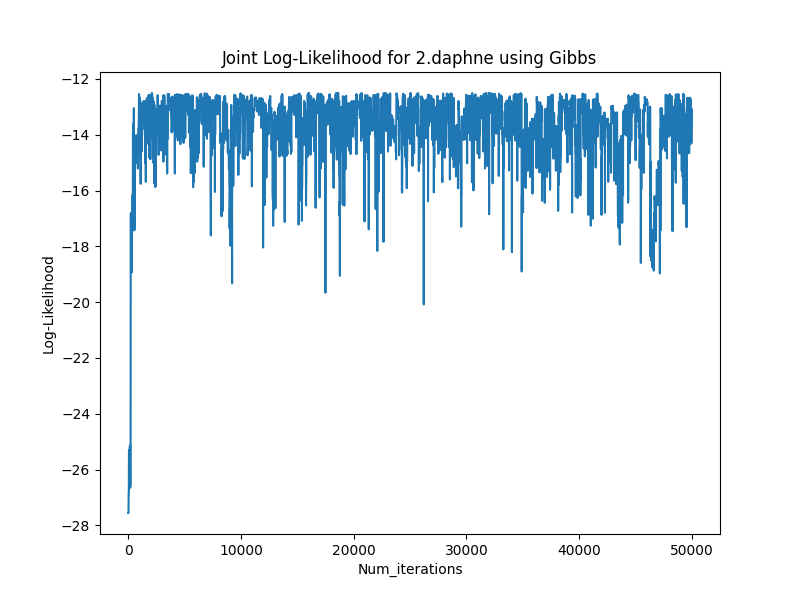
\includegraphics[scale=0.5]{../figs/Gibbs/joint_log_likelihood_2_daphne}
	\caption{Joint Log-likelihood plots for 2.daphne using MH Gibbs Sampling}
\end{figure}

\newpage
\item HMC

\begin{figure}[!ht]
	\centering
	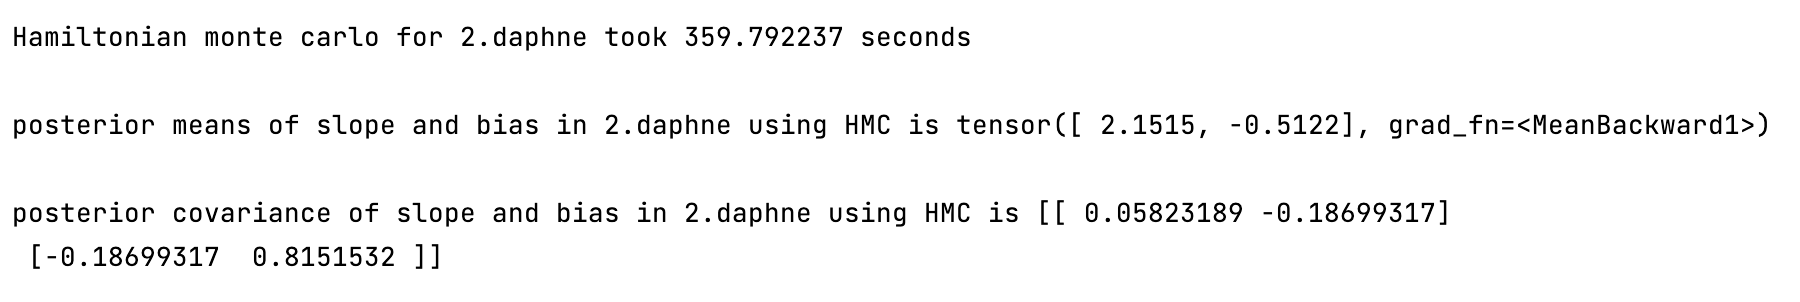
\includegraphics[scale=0.5]{../figs/HMC/2_program_results}
\end{figure}

\begin{figure}[!htp] 
    \centering
    \subfloat[Samples from the posterior for slope]{%
        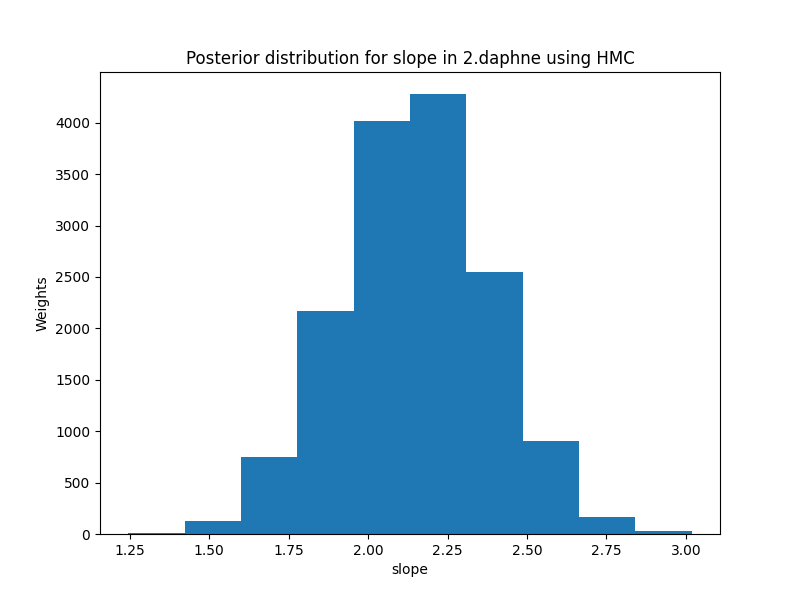
\includegraphics[width=0.5\textwidth]{../figs/HMC/posterior_histogram_slope_2_daphne}%
        \label{fig:a}%
        }%
    \hfill%
    \subfloat[Samples from the posterior for bias]{%
        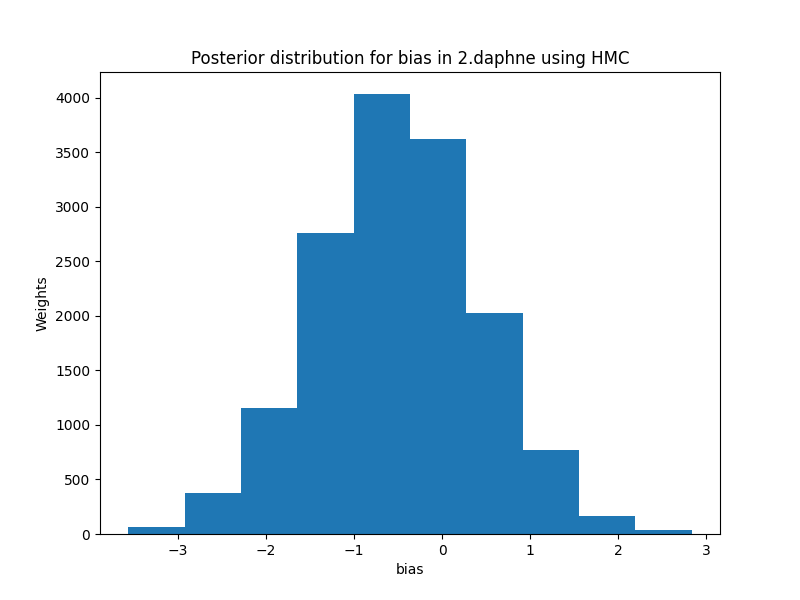
\includegraphics[width=0.5\textwidth]{../figs/HMC/posterior_histogram_bias_2_daphne}%%
        \label{fig:b}%
        }%
        \caption{Posterior distribution for slope and bias for 2.daphne using HMC Sampling}
\end{figure}

\begin{figure}[!htp] 
    \centering
    \subfloat[Samples from the posterior for slope]{%
        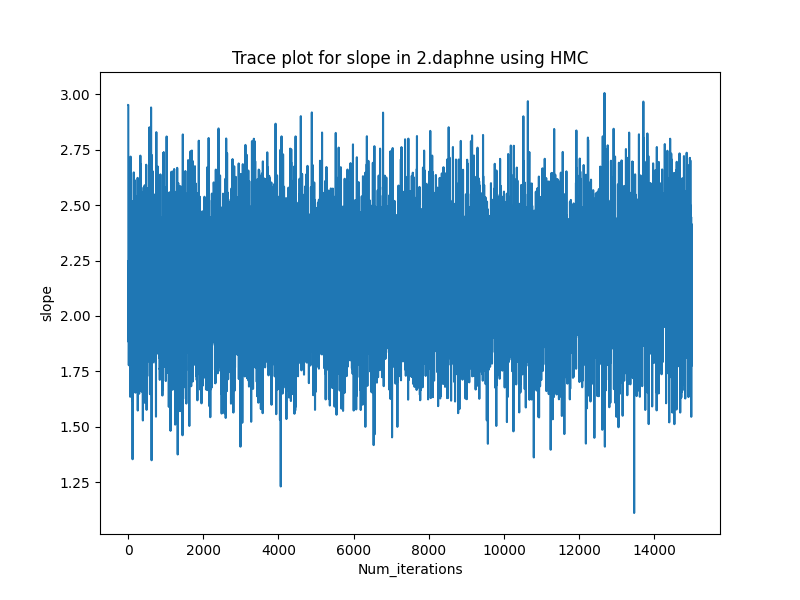
\includegraphics[width=0.5\textwidth]{../figs/HMC/trace_plot_2_slope_daphne}%
        \label{fig:a}%
        }%
    \hfill%
    \subfloat[Samples from the posterior for bias]{%
        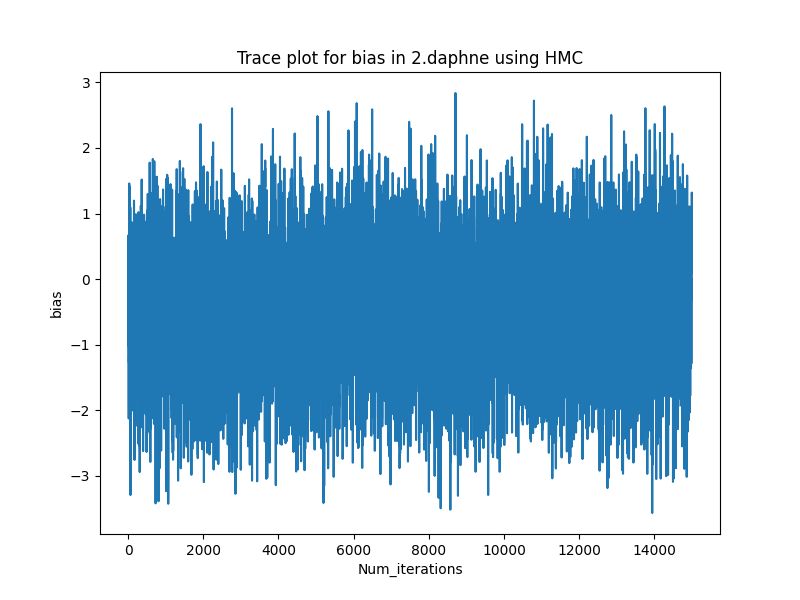
\includegraphics[width=0.5\textwidth]{../figs/HMC/trace_plot_2_bias_daphne}%%
        \label{fig:b}%
        }%
        \caption{Trace plots for slope and bias for 2.daphne using HMC Sampling}
\end{figure}


\begin{figure}[!htp] 
    \centering
    \subfloat[Samples from the posterior for slope]{%
        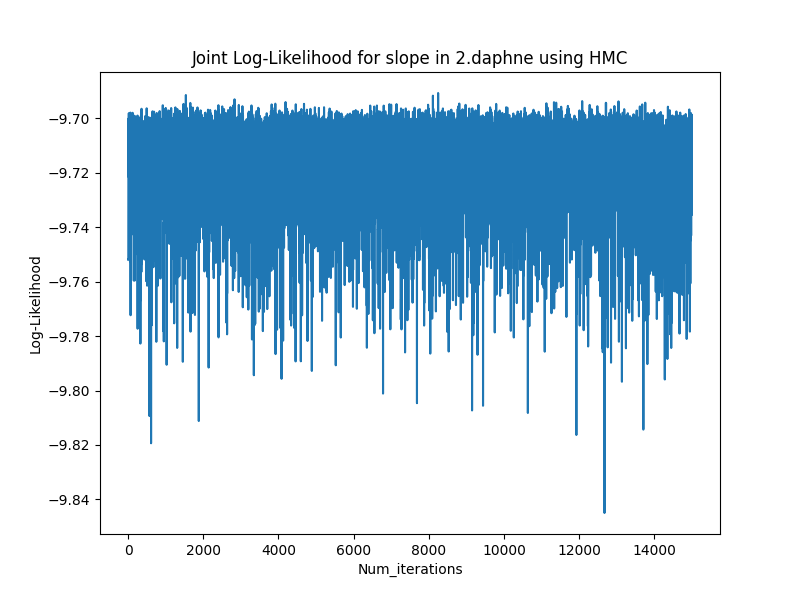
\includegraphics[width=0.5\textwidth]{../figs/HMC/joint_log_likelihood_2_slope_daphne}%
        \label{fig:a}%
        }%
    \hfill%
    \subfloat[Samples from the posterior for bias]{%
        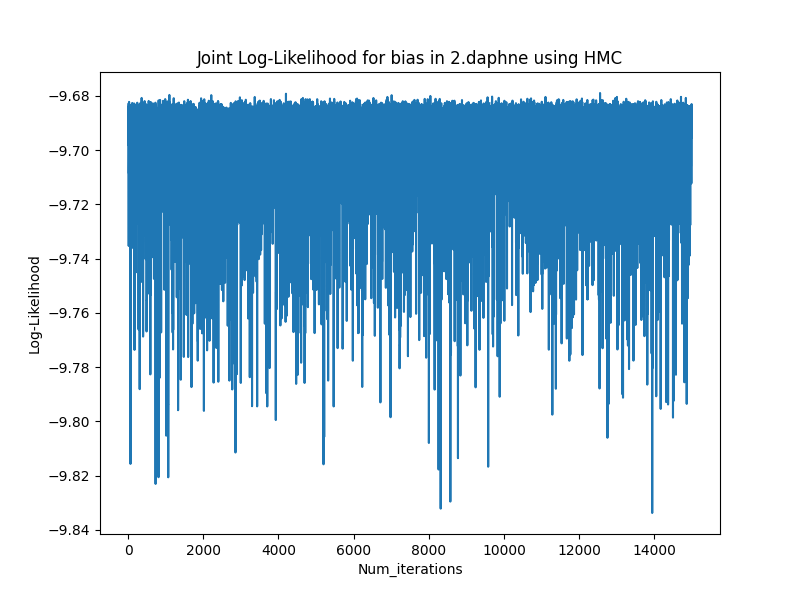
\includegraphics[width=0.5\textwidth]{../figs/HMC/joint_log_likelihood_2_bias_daphne}%%
        \label{fig:b}%
        }%
        \caption{Joint Log-likelihood plots for slope and bias for 2.daphne using HMC Sampling}
\end{figure}

\begin{figure}[!ht]
	\centering
	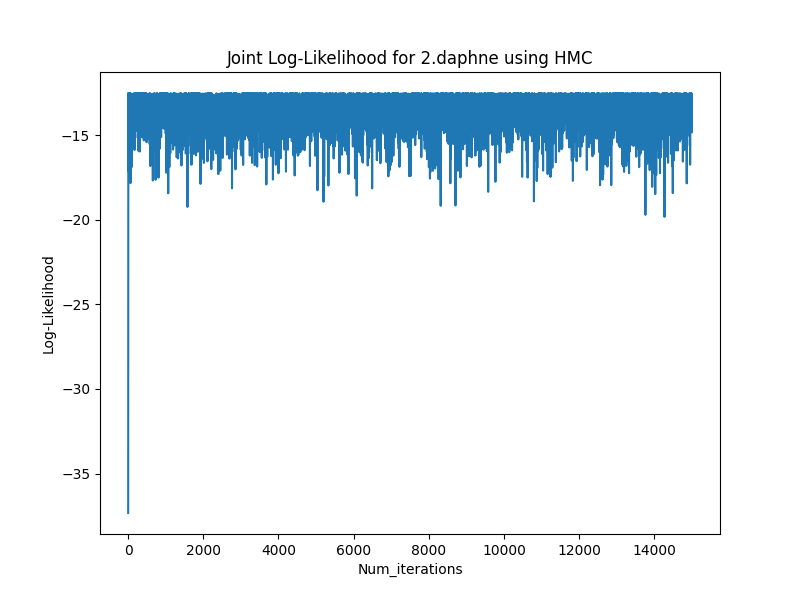
\includegraphics[scale=0.5]{../figs/HMC/joint_log_likelihood_2_daphne}
	 \caption{Joint Log-likelihood plots for 2.daphne using HMC Sampling}
\end{figure}
\end{enumerate}

\newpage
\item Program 3: Importance Sampling was ran 20000 iterations, and Gibbs sampling was ran 10000 iterations.
\begin{enumerate}

\item Importance Sampling

\begin{figure}[!ht]
	\centering
	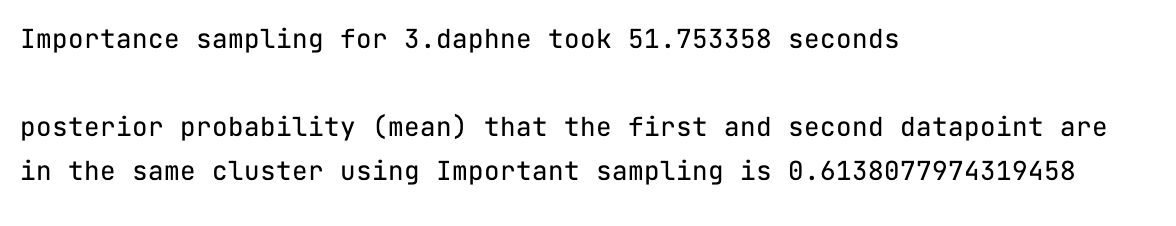
\includegraphics[scale=0.5]{../figs/IS/3_program_results}
\end{figure}

\begin{figure}[!ht]
	\centering
	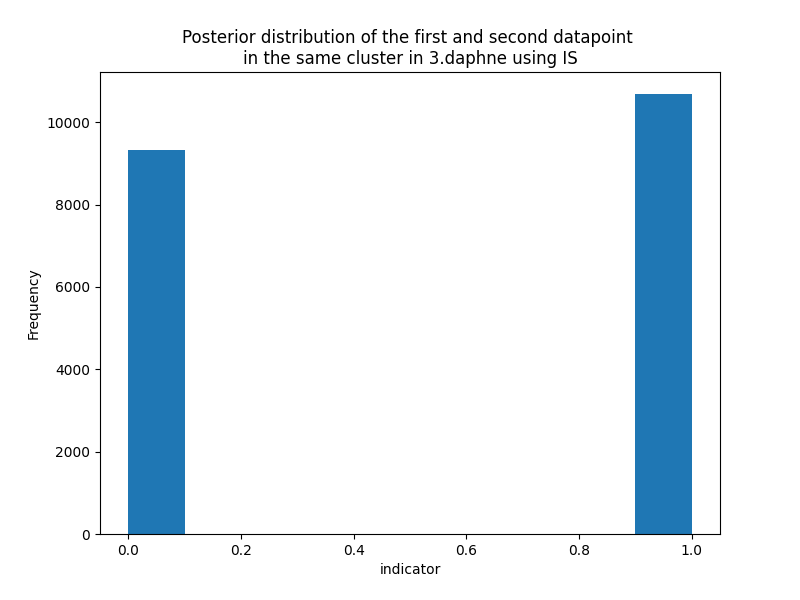
\includegraphics[scale=0.5]{../figs/IS/posterior_histogram_3_daphne}
	 \caption{Posterior distribution for probability for 3.daphne using Importance Sampling}
\end{figure}

\newpage
\item MH Gibbs Sampling

\begin{figure}[!ht]
	\centering
	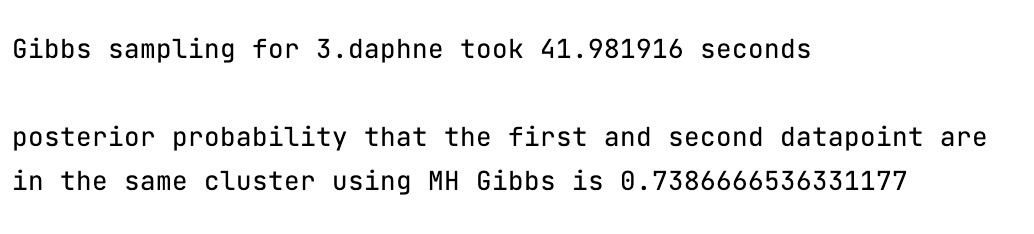
\includegraphics[scale=0.5]{../figs/Gibbs/3_program_results}
\end{figure}

\begin{figure}[!ht]
	\centering
	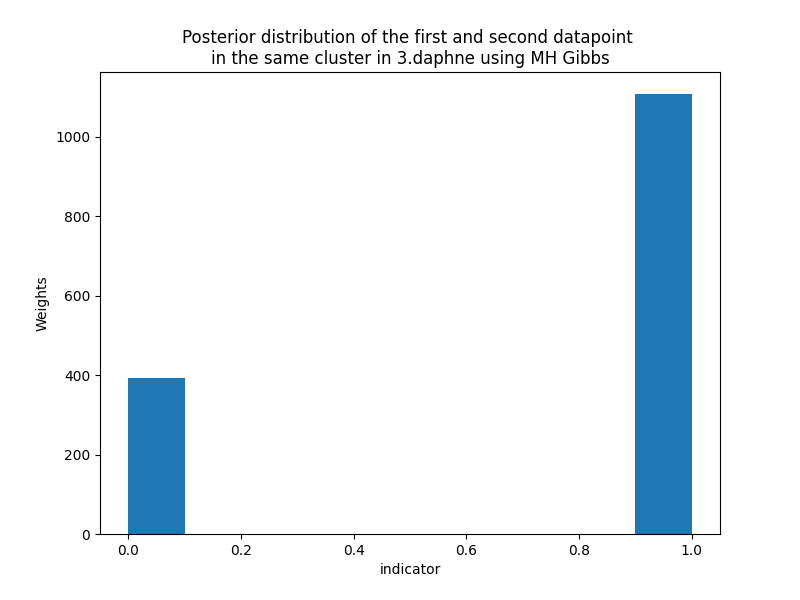
\includegraphics[scale=0.5]{../figs/Gibbs/posterior_histogram_3_daphne}
	 \caption{Posterior distribution for probability for 3.daphne using MH Gibbs Sampling}
\end{figure}

\end{enumerate}

\item Program 4: Both methods were ran 50000 iterations
\begin{enumerate}
\item Importance Sampling

\begin{figure}[!ht]
	\centering
	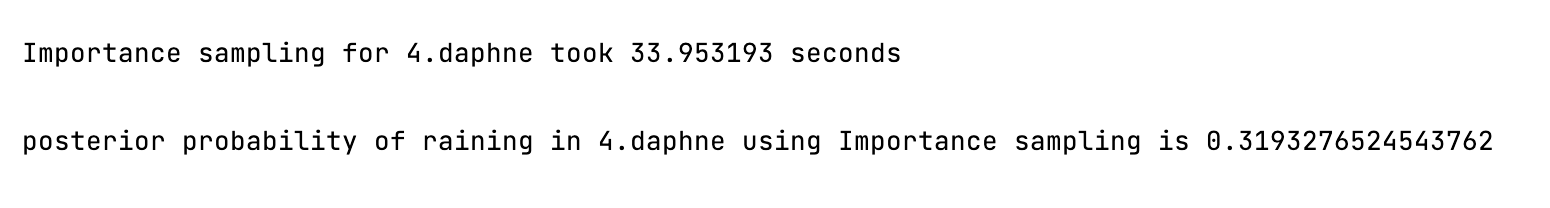
\includegraphics[scale=0.6]{../figs/IS/4_program_results}
\end{figure}

\begin{figure}[!ht]
	\centering
	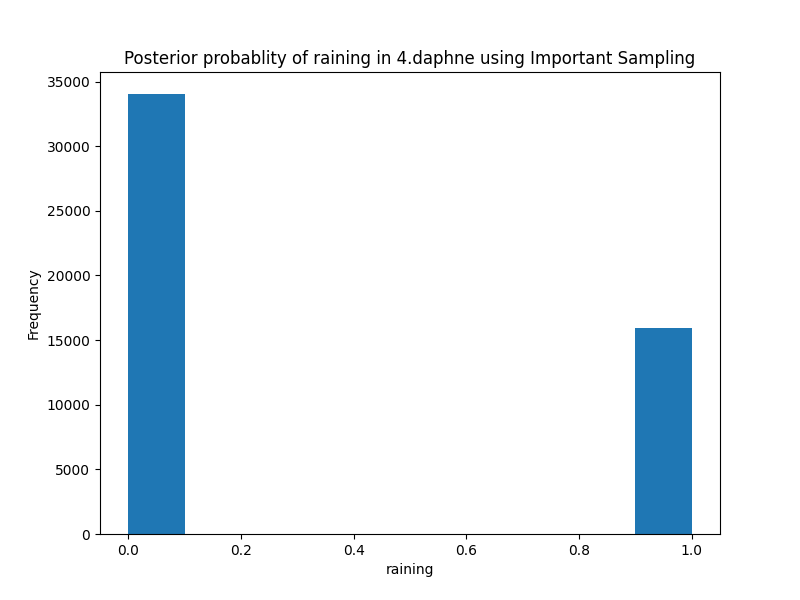
\includegraphics[scale=0.5]{../figs/IS/posterior_histogram_4_daphne}
	 \caption{Posterior distribution for raining for 4.daphne using Importance Sampling}
\end{figure}

\newpage
\item MH Gibb Sampling

\begin{figure}[!ht]
	\centering
	
\includegraphics[scale=0.5]{../figs/Gibbs/4_program_results}
\end{figure}

\begin{figure}[!ht]
	\centering
	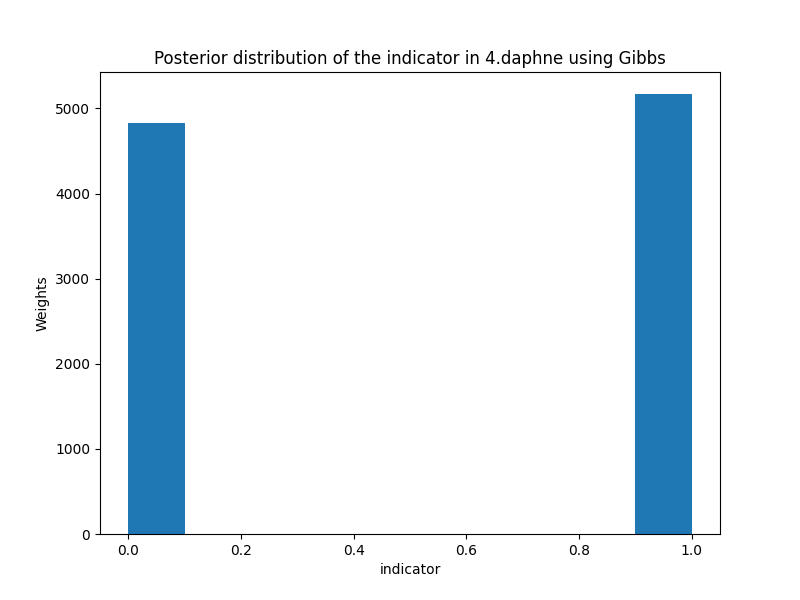
\includegraphics[scale=0.6]{../figs/Gibbs/posterior_histogram_4_daphne}
	\caption{Posterior distribution of raining for 4.daphne using Importance Sampling}
\end{figure}

\end{enumerate}
\newpage
\item The caveat of directly applying Dirac distribution curing sampling process is that the likelihood goes to infinity at the center of the distribution and 0 anywhere else other than the center of the distribution,  such that it is impossible to land into the region that the probability is positive. Therefore,  a function is proposed to approximate Dirac distribution,  which is 
\begin{align*}
f(x) = z\exp(-(x-c)^4)
\end{align*}
where $c$ indicates the center of this function and $z$ is a constant.  It has the similar shape as what Dirac function looks like,  and the highest likelihood also occurs at the center, which is several times of the likelihood corresponding to anywhere else.  More important, this function is differentiable everywhere and also integrable from $-\infty$ to $\infty$:
\begin{align*}
\int_{-\infty}^\infty z\exp(-(x - c)^8\,dx = 2z\Gamma\left(\frac 54\right)z\Rightarrow z = \frac{1}{2\Gamma(5/4)}\ \text{such that the integral is equal to 1}
\end{align*} 
\textbf{Results analysis}: 
\begin{enumerate}
\item Importance Sampling seems giving a good result.  Both posterior means for x and y are around $3.5$ as x and y have the same priors and they are added to approximately $7$.
\item Gibbs Sampling seems giving a not bad result.  The sum of posterior means of x and y is 7 but they are not around $3.5$.  It makes sure that posterior means are on the line $x + y = 7$. This may due to the order that we sample x and y: we sample for x and first and update y based on the resulted value of x.
\item  HMC gives a bad result and it's not efficient.  The gradient could easily go to infinity and samples in the whole process get stuck at some numbers forever so we have to rerun it until the gradients stay at the range of finite numbers with luck.  It's achievable but not reliable to calculate posterior means in this way. 
\end{enumerate}
First two methods were ran 50000 iterations, and HMC was ran 10000 iterations.\\
\hfill
\begin{enumerate}
\item Importance Sampling
\begin{figure}[!ht]
	\centering
	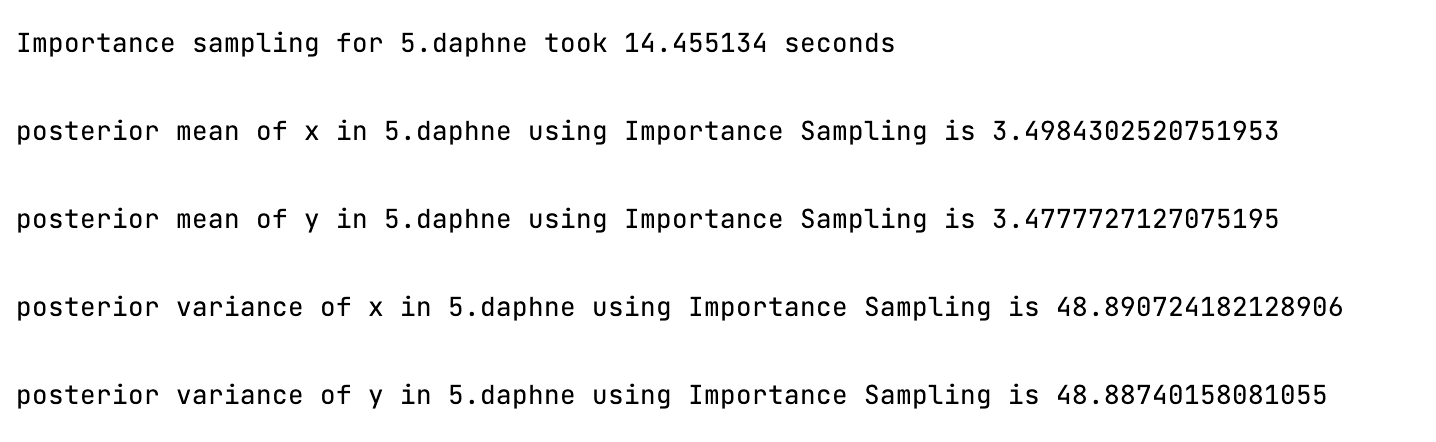
\includegraphics[scale=0.5]{../figs/IS/5_program_results}
\end{figure}

\begin{figure}[!htp] 
    \centering
    \subfloat[Samples from the prior for slope]{%
        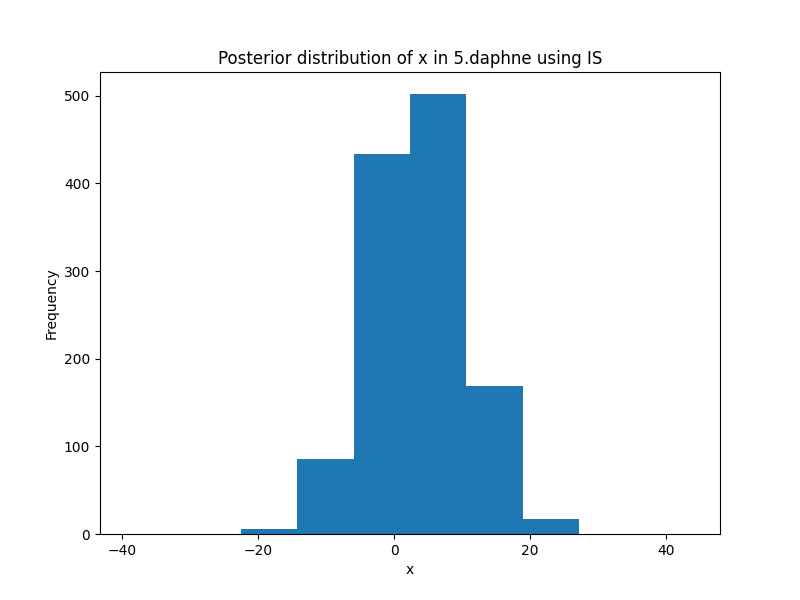
\includegraphics[width=0.5\textwidth]{../figs/IS/posterior_histogram_5_x_daphne}%
        \label{fig:a}%
        }%
    \hfill%
    \subfloat[Samples from the prior for bias]{%
        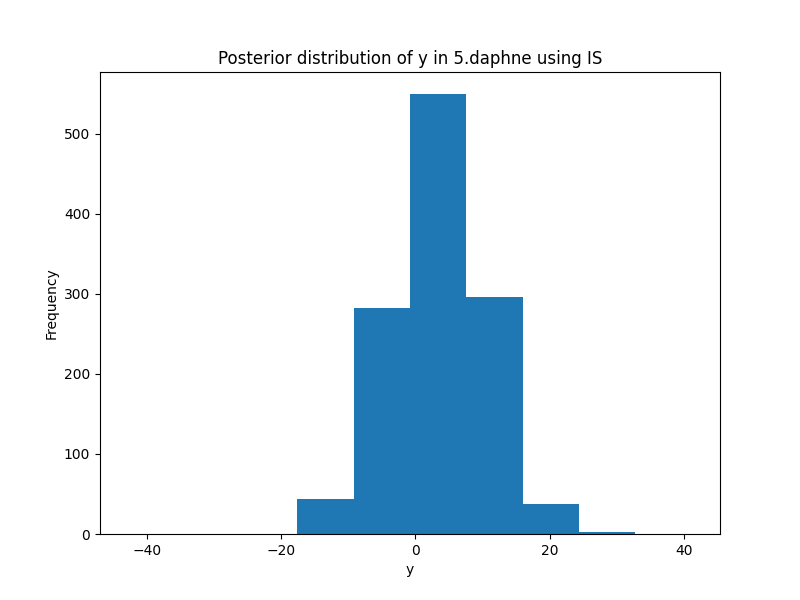
\includegraphics[width=0.5\textwidth]{../figs/IS/posterior_histogram_5_y_daphne}%%
        \label{fig:b}%
        }%
        \caption{Posterior distribution for x and y for 5.daphne using Importance Sampling}
\end{figure}

\newpage
\item MH Gibbs Sampling

\begin{figure}[!ht]
	\centering
	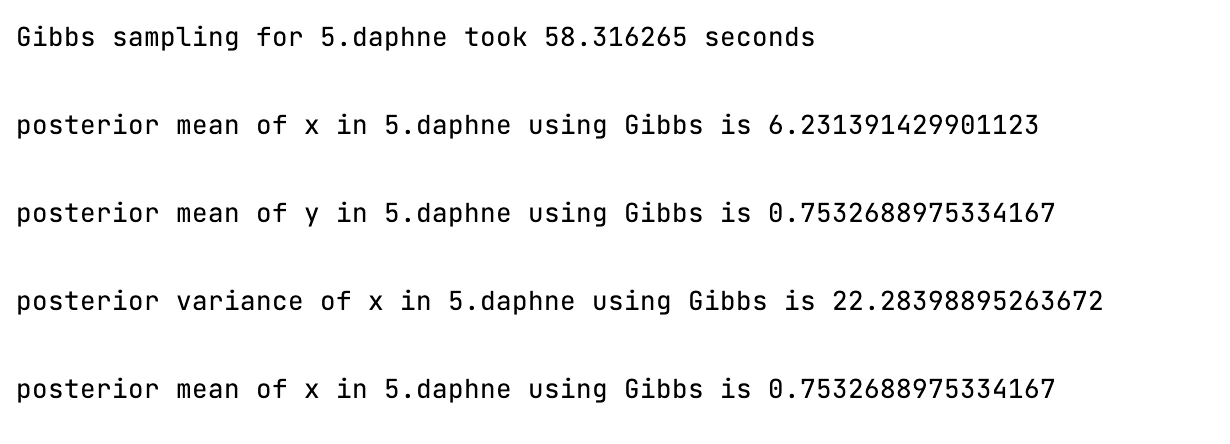
\includegraphics[scale=0.5]{../figs/Gibbs/5_program_results}
\end{figure}

\begin{figure}[!htp] 
    \centering
    \subfloat[Samples from the posterior for slope]{%
        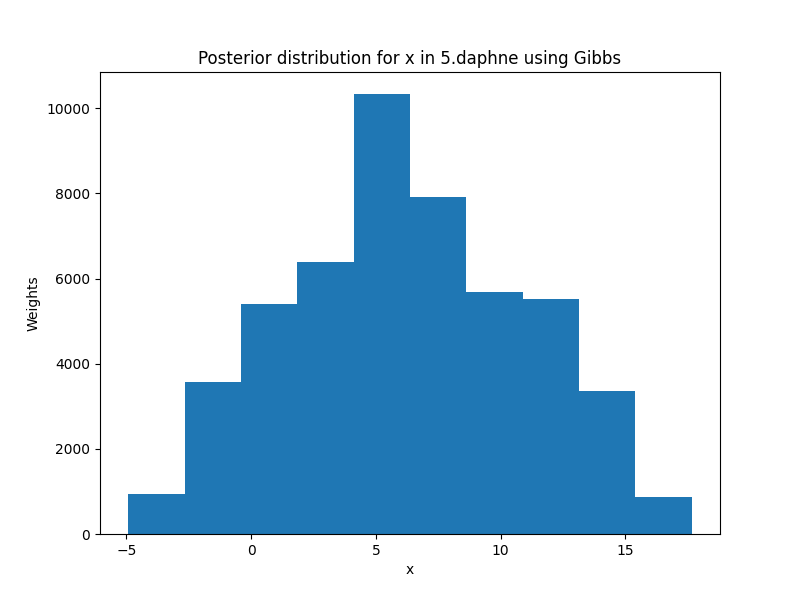
\includegraphics[width=0.5\textwidth]{../figs/Gibbs/posterior_histogram_5_x_daphne}%
        \label{fig:a}%
        }%
    \hfill%
    \subfloat[Samples from the posterior for bias]{%
        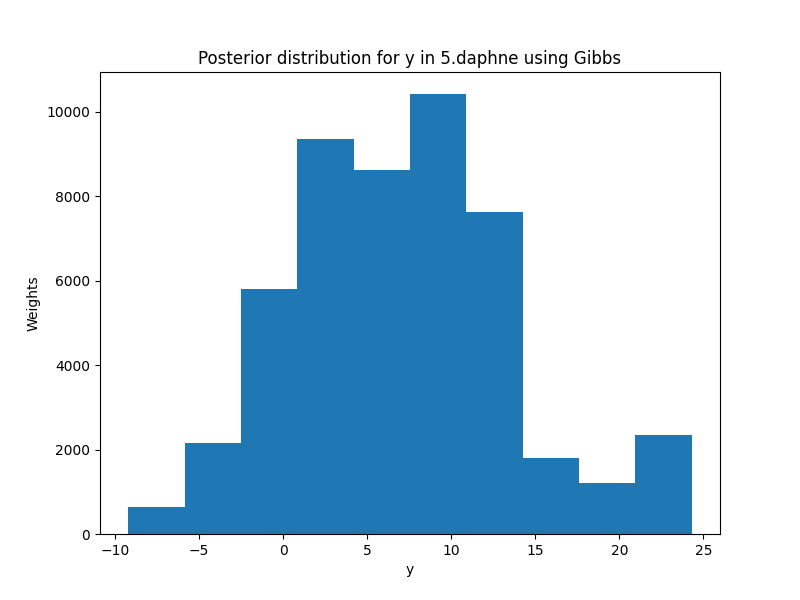
\includegraphics[width=0.5\textwidth]{../figs/Gibbs/posterior_histogram_5_y_daphne}%%
        \label{fig:b}%
        }%
        \caption{Posterior distribution for x and y for 5.daphne using MH Gibbs Sampling}
\end{figure}

\begin{figure}[!htp] 
    \centering
    \subfloat[Samples from the posterior for x]{%
        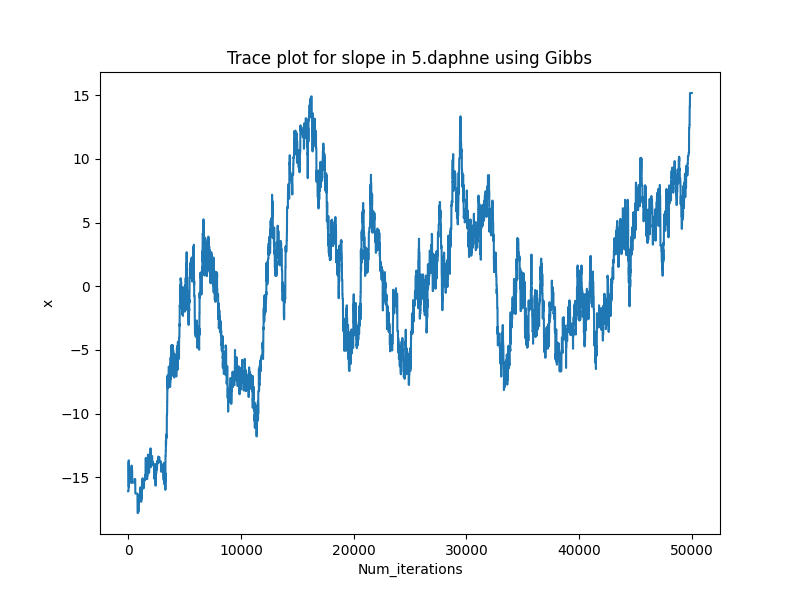
\includegraphics[width=0.5\textwidth]{../figs/Gibbs/trace_plot_5_x_daphne}%
        \label{fig:a}%
        }%
    \hfill%
    \subfloat[Samples from the posterior for y]{%
        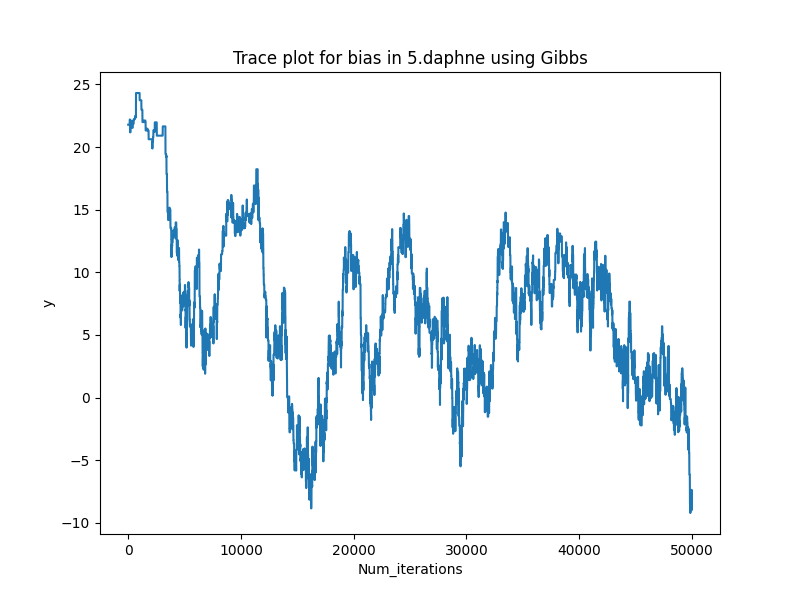
\includegraphics[width=0.5\textwidth]{../figs/Gibbs/trace_plot_5_y_daphne}%%
        \label{fig:b}%
        }%
        \caption{Trace plots for x and y for 5.daphne using MH Gibbs Sampling}
\end{figure}


\begin{figure}[!htp] 
    \centering
    \subfloat[Samples from the posterior for x]{%
        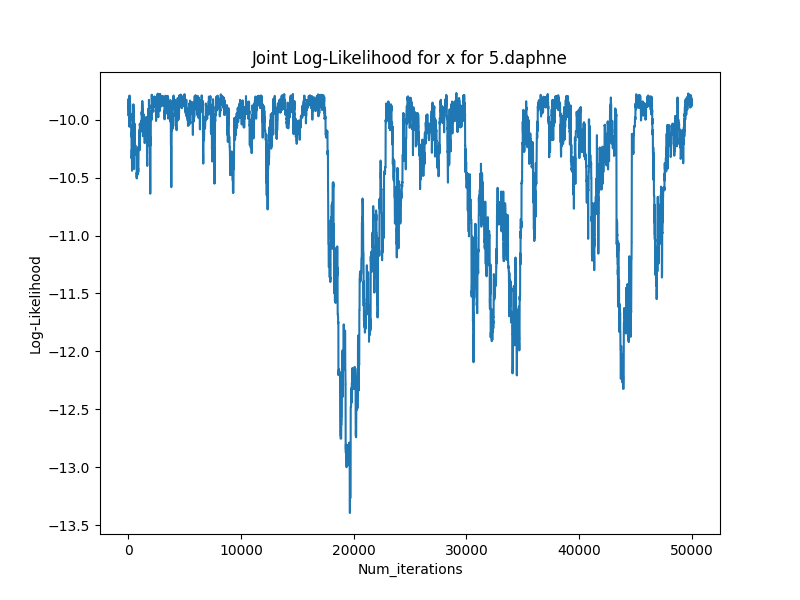
\includegraphics[width=0.5\textwidth]{../figs/Gibbs/joint_log_likelihood_5_x_daphne}%
        \label{fig:a}%
        }%
    \hfill%
    \subfloat[Samples from the posterior for y]{%
        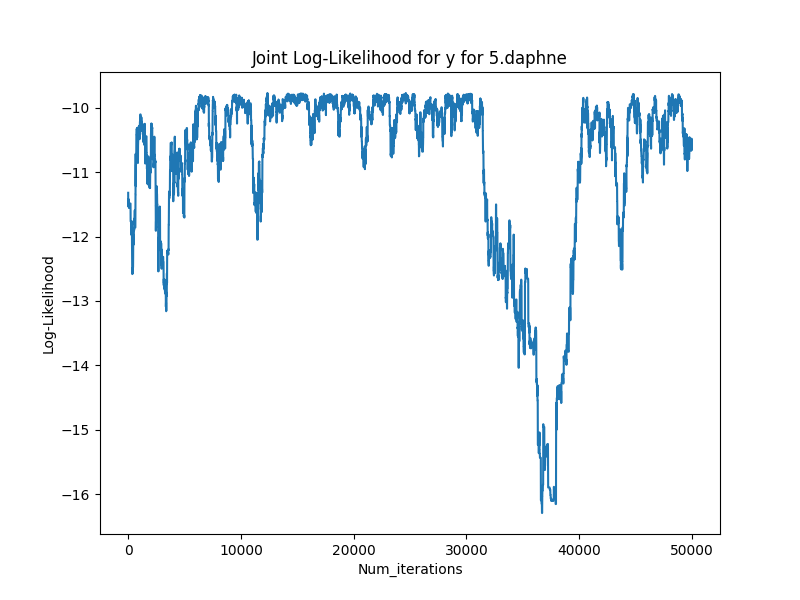
\includegraphics[width=0.5\textwidth]{../figs/Gibbs/joint_log_likelihood_5_y_daphne}%%
        \label{fig:b}%
        }%
        \caption{Joint Log-likelihood plots for x and y for 5.daphne using MH Gibbs Sampling}
\end{figure}

\begin{figure}[!ht]
	\centering
	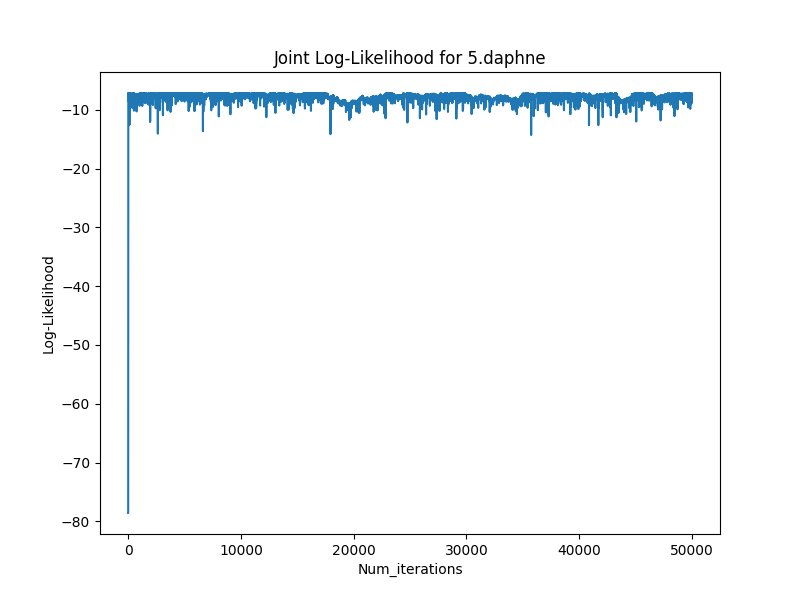
\includegraphics[scale=0.5]{../figs/Gibbs/joint_log_likelihood_5_daphne}
	\caption{Joint Log-likelihood plots for 5.daphne using MH Gibbs Sampling}
\end{figure}

\newpage
\item HMC

\begin{figure}[!ht]
	\centering
	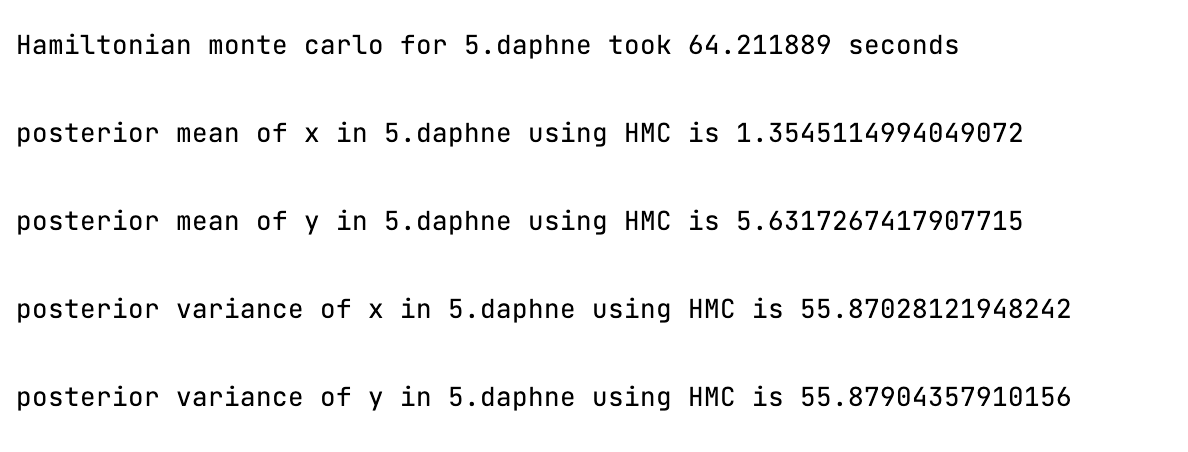
\includegraphics[scale=0.5]{../figs/HMC/5_program_results}
\end{figure}

\begin{figure}[!htp] 
    \centering
    \subfloat[Samples from the posterior for x]{%
        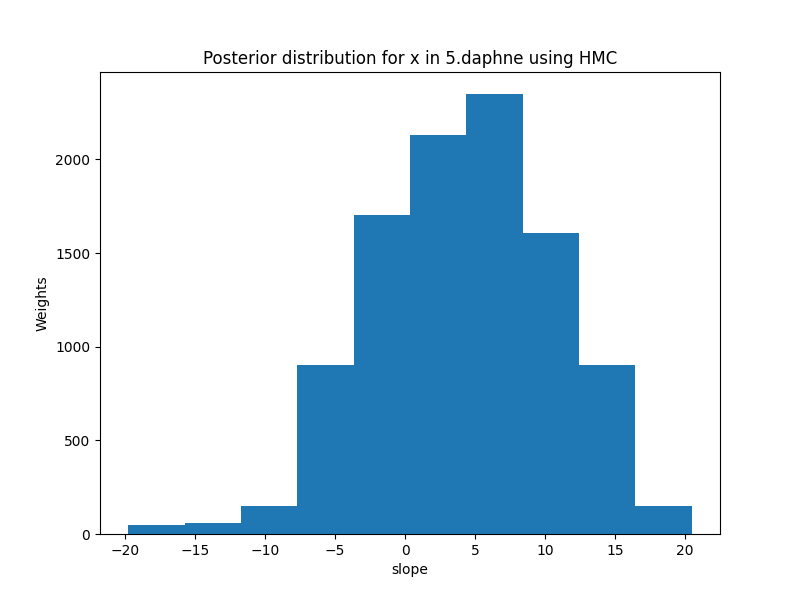
\includegraphics[width=0.5\textwidth]{../figs/HMC/posterior_histogram_5_x_daphne}%
        \label{fig:a}%
        }%
    \hfill%
    \subfloat[Samples from the posterior for y]{%
        \includegraphics[width=0.5\textwidth]{../figs/HMC/posterior_histogram_5_y_daphne}%%
        \label{fig:b}%
        }%
        \caption{Posterior distribution for slope and bias for 5.daphne using HMC Sampling}
\end{figure}

\begin{figure}[!htp] 
    \centering
    \subfloat[Samples from the posterior for x]{%
        \includegraphics[width=0.5\textwidth]{../figs/HMC/trace_plot_5_x_daphne}%
        \label{fig:a}%
        }%
    \hfill%
    \subfloat[Samples from the posterior for y]{%
        \includegraphics[width=0.5\textwidth]{../figs/HMC/trace_plot_5_y_daphne}%%
        \label{fig:b}%
        }%
        \caption{Trace plots for x and y for 5.daphne using HMC Sampling}
\end{figure}


\begin{figure}[!htp] 
    \centering
    \subfloat[Samples from the prior for x]{%
        \includegraphics[width=0.5\textwidth]{../figs/HMC/joint_log_likelihood_5_x_daphne}%
        \label{fig:a}%
        }%
    \hfill%
    \subfloat[Samples from the prior for y]{%
        \includegraphics[width=0.5\textwidth]{../figs/HMC/joint_log_likelihood_5_y_daphne}%%
        \label{fig:b}%
        }%
        \caption{Joint Log-likelihood plots for x and y for 5.daphne using HMC Sampling}
\end{figure}

\begin{figure}[!ht]
	\centering
	\includegraphics[scale=0.5]{../figs/HMC/joint_log_likelihood_5_daphne}
	 \caption{Joint Log-likelihood plots for 5.daphne using HMC Sampling}
\end{figure}
\end{enumerate}

\newpage
\item Code Snippets:

\begin{figure}[!ht]
	\centering
	\includegraphics[scale=0.6]{../figs/IS_1}
	\includegraphics[scale=0.6]{../figs/IS_2}
	\caption{Code for Importance Sampling}
\end{figure}

\begin{figure}[!ht]
	\centering
	\includegraphics[scale=0.5]{../figs/Gibbs_1}
	\caption{Code for MH gibbs sampling Part I}
\end{figure}

\begin{figure}
	\centering
	\includegraphics[scale=0.5]{../figs/Gibbs_2}
	\caption{Code for MH gibbs sampling Part II}
\end{figure}

\begin{figure}
	\centering
	\includegraphics[scale=0.6]{../figs/HMC_1}
	\caption{Code for HMC sampling part I}
\end{figure}

\begin{figure}
	\centering
	\includegraphics[scale=0.6]{../figs/HMC_2}
	\caption{Code for HMC sampling part II}
\end{figure}

\begin{figure}
	\centering
	\includegraphics[scale=0.5]{../figs/HMC_3}
	\caption{Code for HMC sampling part III}
\end{figure}

\end{enumerate}
\end{document}